\section*{Задача 2.1}
Методом простой итерации найти вещественные корни нелинейного уравнения $f(x)=0$ с точностью $\varepsilon = 10^{-8}$.

\[ f(x) = x^3 - 0.9x^2 - x - 0.1. \]

\subsection*{Решение}
Построим график функции и определим отрезки локализации для каждого корня:

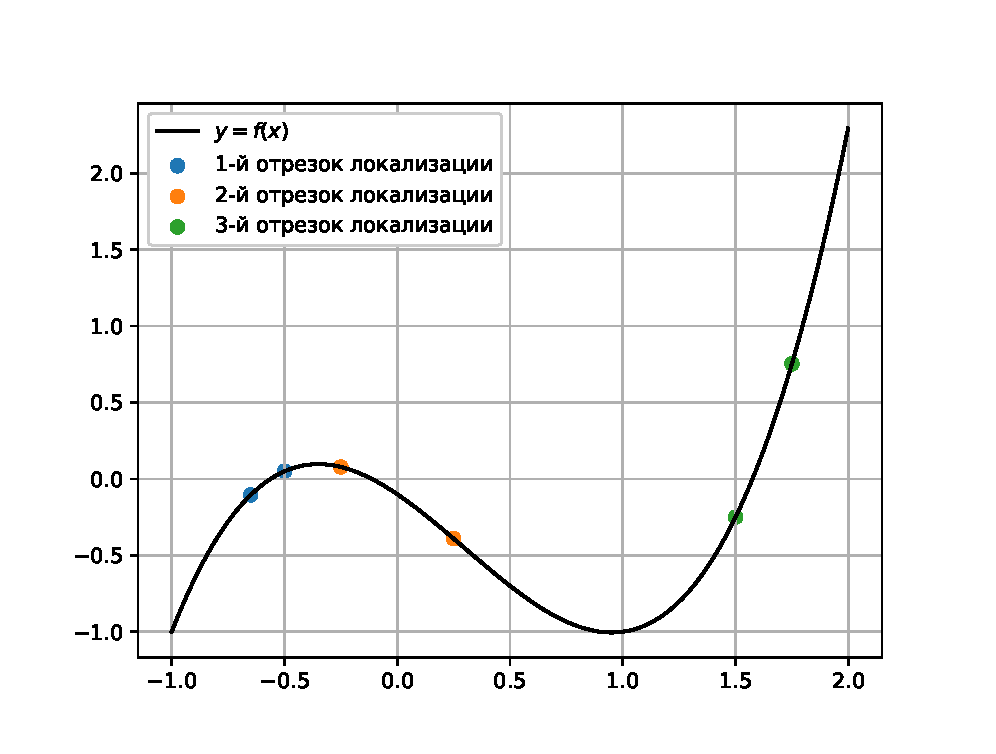
\includegraphics[width=\textwidth]{211.eps}

Определим производную $f(x)$:
\[ f'(x) = 3x^2 - 1.8 x - 1. \]
Построим график производной и отметим на нём границы отрезков локализации:

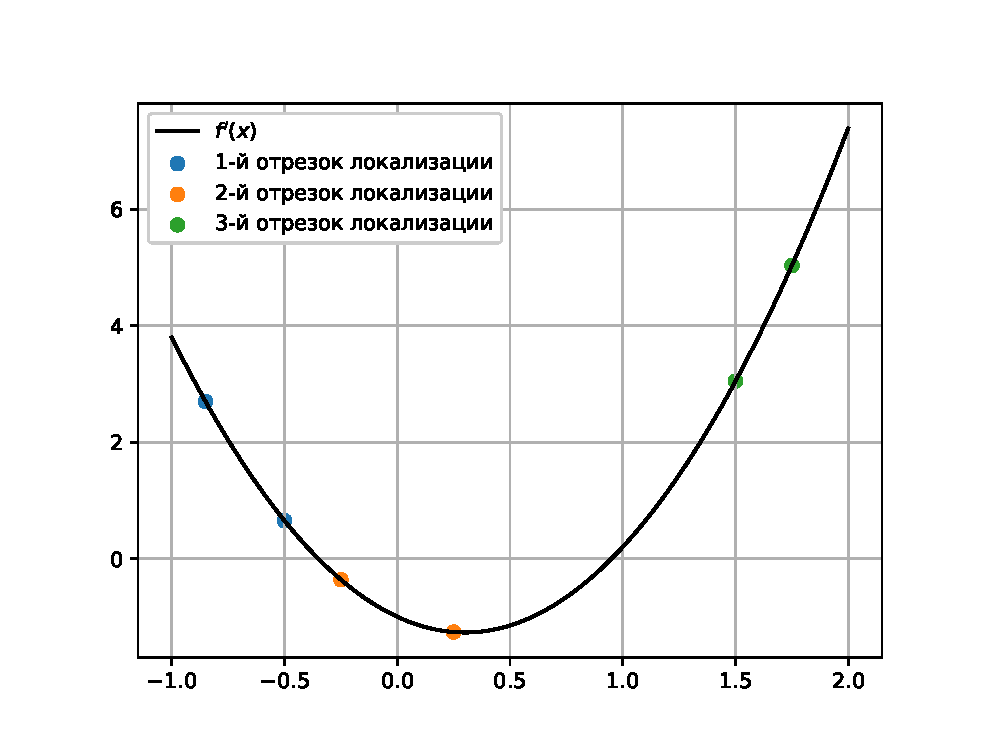
\includegraphics[width=\textwidth]{212.eps}

Из графика видно, что на отрезках локализации производная функции сохраняет постоянный знак.

Для каждого корня определим итерационный параметр $\alpha$ и параметр $q$, используя формулы:
\[ \alpha = \frac{2}{M1 + m1}, \]
\[ q = \left| \frac{M1 - m1}{M1 + m1} \right|, \]
где $M1=\max\limits_{x\in [a,b]} f'(x),\ m1 = \min\limits_{x\in [a,b]}f'(x)$.

Составим программу для нахождения корня с заданной точностью $\varepsilon$ по методу простых итераций. В качестве расчетной формулы используем метод простой итерации с параметром:
\[ x_{n + 1} = x_n - \alpha f(x_n). \]

\begin{verbatim}
def MPI(x0, M1, m1, f, eps):
    alpha = 2 / (M1 + m1)
    q = np.abs((M1 - m1) / (M1 + m1))
    x1 = x0 - alpha * f(x0)
    it = 1
    while abs(x1 - x0) > (1 - q) * eps / q:
        x0, x1 = x1, x1 - alpha * f(x1)
        it += 1
    print(f"Выполнено {it} итераций, x = {x1}")
    return x1
\end{verbatim}

Запишем результаты вычислений в таблицу:

{
\centering
\bgroup
\def\arraystretch{1.5}%
\begin{tabular}{|cccccc|c|}
\hline
\multicolumn{6}{|l|}{Левицкий Валентин Димитриевич A-13-22}                        & Вариант №22            \\ \hline
\multicolumn{6}{|l|}{\( f(x) = x^3 - 0.9x^2 - x - 0.1 \)}                        & \multicolumn{1}{c|}{ \( \varepsilon=10^{-8} \)}  \\ \hline
    \multicolumn{1}{|c|}{Корни}               & \multicolumn{1}{c|}{ \( [a,b] \)}                & \multicolumn{1}{c|}{ \( M_1 \)}          & \multicolumn{1}{c|}{ \( m_1 \)} & \multicolumn{1}{c|}{ \( \alpha \)}   & \multicolumn{1}{c|}{ \( q \)}             & \multicolumn{1}{c|}{Итерации}  \\ \hline
\multicolumn{1}{|c|}{$x_1 = -0.56224597$} & \multicolumn{1}{c|}{$[-0.65, -0.5]$} & \multicolumn{1}{c|}{$1.4375$}  & \multicolumn{1}{c|}{$0.65$}    & \multicolumn{1}{c|}{$0.9581$}  & \multicolumn{1}{c|}{$0.3772$} & \multicolumn{1}{c|}{8} \\
\multicolumn{1}{|c|}{$x_2 = -0.11291429$} & \multicolumn{1}{c|}{$[-0.25, 0.25]$} & \multicolumn{1}{c|}{$-0.3625$} & \multicolumn{1}{c|}{$-1.2625$} & \multicolumn{1}{c|}{$-1.2308$} & \multicolumn{1}{c|}{$0.5538$} & \multicolumn{1}{c|}{8} \\
\multicolumn{1}{|c|}{$x_3= 1.57516025$}   & \multicolumn{1}{c|}{$[1.5, 1.75]$}   & \multicolumn{1}{c|}{$5.0375$}  & \multicolumn{1}{c|}{$3.05$}    & \multicolumn{1}{c|}{$-0.1129$} & \multicolumn{1}{c|}{$1.5752$} & \multicolumn{1}{c|}{8} \\ \hline
\end{tabular}
\egroup
}
